\chapter{Finite Element Neutron Diffusion}
\label{ch:neutronDiffusion}

\section{Introduction}
  For typical nuclear reactor applications, diffusion theory well approximates 
  the neutron distribution within the reactor. The neutron diffusion equation is
  a second order partial differential equation in space and energy. In standard
  notation, the continuous neutron diffusion equation is presented as
  \begin{multline}\label{eq:continuous_diffusion}
    -\grad \cdot (D(\vr,E) \grad \phi(\vr,E)) + \Sigma_t(\vr,E) \phi(\vr,E) = \\
      \frac{\chi(\vr,E)}{\keff} \int_0^{\infty} \nu_f(\vr,E') \Sigma_f(\vr,E') 
      \phi(\vr,E') \; dE' + \int_0^{\infty} \Sigma_s(\vr,E' \rightarrow E) 
      \phi(\vr,E') \; dE'
  \end{multline}
  Where $D$ is the diffusion constant, $\phi$ is the scalar neutron flux, 
  $\Sigma_t$ is the total cross section, $\chi$ is the fission neutron 
  spectrum, $\keff$ is the effective neutron multiplication factor, $\Sigma_f$ 
  is the fission cross section, $\nu_f$ is the neutron yield per fission, and 
  $\Sigma_s(\vr,E' \rightarrow E)$ is the scattering cross section for neutrons 
  at position $\vr$ scattering from energy $E'$ to $E$.
  
  The neutron diffusion equation must be discretized in space and 
  energy to be solved numerically. Energy discretization is relatively 
  straight-forward and is performed using the multigroup method. Spatial 
  discretization requires more attention and will be done with the Finite 
  Element Method (FEM). This method is selected for several reasons. It allows
  for easily increasing the order of the method by increasing the order of the 
  elements with no changing of the mesh required. Coordinates of nodes can be 
  easily updated to reflect physical phenomena such as thermal expansion 
  (\chref{ch:thermalExpansion}). Additionally, material properties are 
  calculated on an element basis allowing for fine detail updates to the 
  material properties during the calculation.
  
  For energy discretization, An energy structure is described as $\{E_g\}$ for 
  $g = 1,2,\ldots,G$ and by convention
  \[ E_G > E_{G-1} > \ldots > E_2 > E_1  \]
  Then, multigroup constants can be calculated based on the energy group 
  structure and the known cross sections. Multigroup constants are calculated to
  preserve the number of neutrons produced or destroyed. That is, the 
  calculation preserves reaction rates where the reaction rate for reaction $x$
  is defined as $R_x=\Sigma_x \phi$. Multigroup constants are then calculated. A
  formal derivation is given in \cite{duderstathamilton} and the results are 
  presented below.
  \begin{align}
    D_g(\vr) &= \frac{\int_{E_g}^{E_{g-1}} D(\vr,E') \grad \phi(\vr,E)\;dE}
      {\int_{E_g}^{E_{g-1}} \grad \phi(\vr,E)\;dE} \\
    \Sigma_{t,g}(\vr) &= \frac{\int_{E_g}^{E_{g-1}} \Sigma_t(\vr,E) 
      \phi(\vr,E)\;dE}{\int_{E_g}^{E_{g-1}} \phi(\vr,E)\;dE} \\
    \nu\Sigma_{f,g}(\vr) &= \frac{\int_{E_g}^{E_{g-1}} \nu_f(\vr,E)
      \Sigma_f(\vr,E) \phi(\vr,E)\;dE}{\int_{E_g}^{E_{g-1}} 
      \phi(\vr,E)\;dE} \\
    \Sigma_{s,g\rightarrow g'}(\vr) &= \frac{\int_{E_g'}^{E_{g'-1}} 
      \int_{E_g}^{E_{g-1}} \Sigma_s(\vr,E' \rightarrow E) \phi(\vr,E')\;dE\;dE'}
      {\int_{E_g}^{E_{g-1}} \phi(\vr,E)\;dE}  \\
    \chi_g(\vr) &= \int_{E_g}^{E_{g-1}} \chi(\vr,E) \; dE \\
    \phi_g(\vr) &= \int_{E_g}^{E_{g-1}} \phi(\vr,E) \; dE
  \end{align}
  Note that cross sections $\nu_f(\vr,E)$ and $\Sigma_f(\vr,E)$ have been 
  combined. This is necessary and a mathematical result of the group collapse.
  Then, \eref{eq:continuous_diffusion} can be discretized in energy as
  \begin{align}\label{eq:multigroup_diffusion}
    - \grad \cdot ( D_g(\vr) \grad \phi_g(\vr)) + \Sigma_{t,g}(\vr) \phi_g(\vr)= 
      \frac{\chi_g(\vr)}{\keff} \sum_{g'=1}^{G} \nu\Sigma_{f,g'}(\vr) 
      \phi_{g'}(\vr) + \sum_{g'=1}^{G} \Sigma_{s,g' \rightarrow g}(\vr) 
      \phi_{g'}(\vr)
  \end{align}
  The neutron diffusion equation has now been discretized in energy.
  Spatial dicretization will be based on the Finite Element Method (FEM) and 
  will be discussed in \sref{sec:formulation:derivation}.
  
  % todo this discussion may need to be moved to 'Implementation'
  The total neutron cross section includes the contribution due to 
  self-scattering. That is, due to $\Sigma_{s,g\rightarrow g}$. This can be 
  removed from \eref{eq:multigroup_diffusion} for simplicity.
  \begin{equation} \label{eq:multigroup_removal}
    - \grad \cdot( D_g(\vr) \grad \phi_g(\vr)) + \Sigma_{r,g}(\vr) \phi_g(\vr) = 
      \frac{\chi_g(\vr)}{\keff} \sum_{g'=1}^{G} \nu\Sigma_{f,g'}(\vr) 
      \phi_{g'}(\vr) + \sum_{g'=1, g' \ne g}^{G} \Sigma_{s,g' \rightarrow g}(\vr) 
      \phi_{g'}(\vr)
  \end{equation}
  Where $\Sigma_{r,g}$ is the removal cross section and $\Sigma_{r,g}(\vr) = 
  \Sigma_{t,g}(\vr) - \Sigma_{s,g\rightarrow g}(\vr)$. For simplicity, the
  neutron sources in \eref{eq:multigroup_removal} can be  combined into a
  single term.
  \begin{equation} \label{eq:multigroup_source}
    - \grad \cdot( D_g(\vr) \grad \phi_g(\vr)) + \Sigma_{r,g}(\vr) \phi_g(\vr) = 
      q_g(\vr)
  \end{equation}
  Where $q_g(\vr)$ is the combined neutron source at position $\vr$. $q$ can 
  then be further divided into contributions due to fission ($q_{fiss}$), 
  up- scattering ($q_{up}$) when a neutron increases in energy, and 
  down-scattering when a neutron decreases in energy ($q_{down}$).
  \begin{align}
    q_g(\vr) &= q_{fiss,g}(\vr) + q_{up,g}(\vr) + q_{down,g}(\vr) \\
    q_{fiss,g}(\vr) &= \frac{\chi_g(\vr)}{\keff} \sum_{g'=1}^{G} 
      \nu \Sigma_{f,g'}(\vr) \phi_{g'}(\vr) \\
    q_{up,g}(\vr) &= \sum_{g'=g+1}^{G} \Sigma_{s,g' \rightarrow g}(\vr)
      \phi_{g'}(\vr) \\
    q_{down,g}(\vr) &= \sum_{g'=1}^{g} \Sigma_{s,g' \rightarrow g}(\vr)
      \phi_{g'}(\vr)
  \end{align}
  Where the difference between $q_{up}$ and $q_{down}$ are the limits of the 
  summation. This form allows for operator splitting of the neutron source term.
  In an iterative scheme, it will be necessary for fission and up-scatter 
  sources to use a different flux iterate than down-scatter so this division
  will prove useful.
  

\section{Formulation}
  \subsection{Derivation}
    \label{sec:formulation:derivation}
    The only remaining continuous variable in the problem is the spatial 
    variable $\vr$. This will be discretized according to the Finite Element 
    Method (FEM). The form of the diffusion equation to be discretized is 
    \eref{eq:multigroup_source}. The problem is solved in a finite domain 
    $\vr \in \Omega$ where $\partial \Omega$ represents the boundary of the 
    domain where some boundary condition is specified. Boundary condition 
    options provided include
    \begin{enumerate}
      \item Mirror. $\grad \phi_g(\vr) = 0$ for $\vr \in \partial \Omega$.
      \item Albedo. $D_g(\vr) \grad \phi_g(\vr) + \albedo \phi_g(\vr)=0$ for 
        $\vr \in \partial \Omega$ where $\albedo$ is a real constant specified
        by the user. For vacuum conditions, $\alpha = \half$.
      \item Zero Flux. $\phi_g(\vr) = 0$ for $\vr \in \partial \Omega$.
    \end{enumerate}
    (Note: the order of the above list corresponds to the order of boundary 
    condition precedent in code with the greater the integer, the greater the 
    precedent.)
    
    Finite Element derivation begins with \eref{eq:multigroup_source}.
    The equation is multiplied by a testing function $v(\vr) \in H_1(\Omega)$ 
    Where $H$ is the Sobolev Space. Then, the equation is integrated over the 
    problem domain. This yields the Weak Form or Variational Form of the 
    problem.
    \begin{align}
      -\grad \cdot (D_g(\vr) \grad \phi_g(\vr)) + \Sigma_{r,g}(\vr) \phi_g(\vr)
        &=q_g(\vr) \\
      -\grad \cdot (D_g(\vr) \grad \phi_g(\vr)) v(\vr) + 
        \Sigma_{r,g}(\vr) \phi_g(\vr) v(\vr) &=
        q_g(\vr) \\
      - \int_{\Omega} \grad \cdot (D_g(\vr) \grad \phi_g(\vr)) v(\vr) \; d\Omega
        \int_{\Omega} \Sigma_{r,g}(\vr) \phi_g(\vr) v(\vr) \;d\Omega &=
        \int_{\Omega} q_g(\vr) v(\vr) \;d\Omega
    \end{align}
    
    For the purposes of this application, material cross sections and the
    neutron source are assumed to be constant within an element. Then, the 
    integral can be partitioned into a sum of integrals over the elements in the
    domain assuming the set of elements $\{\Omega_e\} = \Omega$ for 
    $e = 1,2,\ldots,E$ where $E$ is the total number of elements.
    \begin{equation} \label{eq:element_by_element}
      -\sum_{e=1}^{E} D_{g,e} 
        \int_{\Omega_e} \grad \cdot \grad \phi_g(\vr) v(\vr) \; d\Omega_e +
        \sum_{e=1}^{E} \Sigma_{r,g,e} \int_{\Omega_e} \phi_g(\vr) v(\vr) 
        \;d\Omega_e = \sum_{e=1}^{E} q_{g,e} \int_{\Omega_e} v(\vr) 
        \; d\Omega_e
    \end{equation}
    The Second Green's Theorem is used to simplify the integral in the first
    term. A proof can be found in \cite{textbookli} in Theorem 9.2.
    \begin{equation} \label{eq:greens}
      -\int_{\Omega_e} \grad \cdot \grad \phi_g(\vr) v(\vr) \;d\Omega_e =
        -\int_{\partial \Omega_e}  
        \frac{\partial \phi_g(\vr)}{\partial \vn} v(\vr)\; ds + \int_{\Omega_e} 
        \grad \phi_g(\vr) \cdot \grad v(\vr) \; d\Omega_e
    \end{equation}
    Where $\frac{\partial \phi_g(\vr)}{\partial \vn}$ is the outward normal 
    derivative and the integral $ds$ is a line integral in two dimensions or a 
    surface integral in three dimensions. Recognizing that this quantity will 
    only be relevant on the boundary of the problem, the value of the outward 
    normal derivative may be specified in a boundary condition. Specifically, 
    the Albedo boundary condition which has the following form for $\vr \in 
    \partial \Omega$. 
    \begin{align}
      D_g(\vr) \grad \phi_g(\vr) + \albedo \phi_g(\vr) &= 0 \\
      \grad \phi_g(\vr) &= \frac{-\albedo \phi_g(\vr)}{D_g}
    \end{align}
    Substituting \eref{eq:greens} into  \eref{eq:element_by_element} and 
    assuming the outward normal derivative is specified in the form of an Albedo
    boundary condition.
    \begin{multline} 
      -\sum_{e=1}^{E} D_{g,e} \int_{\partial \Omega_e} v(\vr) 
        \frac{\partial \phi_g(\vr)}{\partial \vn} \;ds + \sum_{e=1}^{E} D_{g,e}
        \int_{\Omega_e} \grad \phi_g(\vr) \cdot \grad v(\vr) \; d\Omega_e + \\
        \sum_{e=1}^{E} \Sigma_{r,g,e} \int_{\Omega_e} \phi_g(\vr) v(\vr) 
        \; d\Omega_e =
        \sum_{e=1}^{E} q_{g,e} \int_{\Omega_e} v(\vr) \; d\Omega_e
    \end{multline}
    \begin{multline} \label{eq:element_boundary}
      \sum_{e=1}^{E} \albedo \int_{\partial \Omega_e} v(\vr) 
        \phi_g(\vr) \;ds + \sum_{e=1}^{E} D_{g,e}
        \int_{\Omega_e} \grad \phi_g(\vr) \cdot \grad v(\vr) \; d\Omega_e + \\
        \sum_{e=1}^{E} \Sigma_{r,g,e} \int_{\Omega_e} \phi_g(\vr) v(\vr) 
        \; d\Omega_e =
        \sum_{e=1}^{E} q_{g,e} \int_{\Omega_e} v(\vr) \; d\Omega_e
    \end{multline}
    Now the function of interest $\phi_g(\vr)$ is assumed to be a linear 
    combination of chosen basis functions $\{\basis_i\}$.
    \begin{equation} \label{eq:linear_combination}
      \phi_g(\vr) = \sum_{i=1}^{N} \alpha_{g,i} \basis_i(\vr)
    \end{equation}
    Where coefficients $\{\alpha_i\}$ are unknown and will be determined. 
    Typically, these basis functions have unit magnitude and are centered at the
    node  points so the coefficients $\alpha_i$ are the approximated solution at
    the nodes. Basis functions are typically polynomials of arbitrary magnitude. 
    Linear and quadratic polynomials are common but for the application 
    presented here, only linear basis functions are explored.
    The test function $v(\vr)$ is also chosen as a linear combination of the 
    basis functions.
    \begin{equation} \label{eq:linear_superposition}
      v(\vr) = \sum_{j=1}^{N} \basis_j(\vr)
    \end{equation}
    The testing function is arbitrary so the magnitude is fixed to the magnitude
    of the basis function.
    
    \eref{eq:linear_combination} and \eref{eq:linear_superposition} are plugged
    into \eref{eq:element_boundary}. This yields a linear system of equations.
    \begin{multline}
      \sum_{e=1}^{E} \albedo \sum_{i=1}^{N} \alpha_{i,g}
        \int_{\partial \Omega_e}
        \basis_i(\vr)  \basis_j(\vr) \;ds +
        \sum_{e=1}^{E} D_{g,e} \sum_{i=1}^{N} \alpha_{i,g}
        \int_{\Omega_e} \grad \basis_i(\vr) \cdot \grad \basis_i(\vr)\;d\Omega_e
        + \\
        \sum_{e=1}^{E} \Sigma_{r,g,e} \sum_{i=1}^{N} \alpha_{i,g}
        \int_{\Omega_e} \basis_i(\vr) \basis_i(\vr) \; d\Omega_e =
        \sum_{e=1}^{E} q_{g,e} \sum_{i=1}^{N} 
        \int_{\Omega_e} \basis_i(\vr) \; d\Omega_e
    \end{multline}
    \begin{multline}
      \sum_{i=1}^{N} \alpha_{i,g} \sum_{j=1}^{N} \left(
        \sum_{e=1}^{E} \albedo \int_{\partial \Omega_e}
        \basis_i(\vr)  \basis_j(\vr) \;ds +
        \sum_{e=1}^{E} D_{g,e} 
        \int_{\Omega_e} \grad \basis_i(\vr) \cdot \grad \basis_j(\vr)\;d\Omega_e
        \right.
        + \\
        \left.
        \sum_{e=1}^{E} \Sigma_{r,g,e}
        \int_{\Omega_e} \basis_i(\vr) \basis_j(\vr) \; d\Omega_e \right) =
        \sum_{i=1}^{N} \left(
        \sum_{e=1}^{E} q_{g,e} 
        \int_{\Omega_e} \basis_i(\vr) \; d\Omega_e \right)
    \end{multline}
    \begin{align}
      \label{eq:fem_notation}
      a(\basis_i,\basis_j) &= f(\basis_i) \\
      \ma \vu &= \vf
    \end{align}
    $a(\basis_i,\basis_j)$ is the bilinear form and $f(\basis_i)$ is the linear 
    form of the finite element system. The notation of \eref{eq:fem_notation} is
    common to mathematical discussions of the FEM. The diffusion coefficient 
    $D_g(\vr)$ is nonzero and bounded and the removal cross section 
    $\Sigma_{r,g}(\vr)$ is bounded. Theorem 9.3 \cite{textbookli} then shows 
    that the finite element equations satisfy the Lax-Milgram Lemma implying 
    the solution to the finite element method are unique and bounded. This is 
    not purely the case as the source function $q_g(\vr)$ is updated on each 
    iteration. In each iteration a unique solution exists. The global problem
    remains an eigenvalue problem as described in \cite{duderstathamilton}. The
    method will return the fundamental eigenvalue $\keff$ and the shape function
    which must be normalized by an arbitrary constant.
    
    In matrix notation, $\ma$ is described by the integral quantities (more to 
    follow),  $\vu = \{\alpha_i\}$, and $\vf$ is described by the source 
    integral quantity. Inspecting the matrix $\ma$ and the vector $\vf$ reveals 
    the following.
    \begin{align}
      \label{eq:matrix_population}
      A_{i,j,g,e} &= \albedo \int_{\partial \Omega_e} \basis_i(\vr) 
        \basis_j(\vr) \; ds + D_{g,e} 
        \int_{\Omega_e} \grad \basis_i(\vr) \cdot \grad \basis_j(\vr) \;
        d\Omega_e + \Sigma_{r,g,e} \int_{\Omega_e} \basis_i(\vr) \basis_j(\vr)
        \; d\Omega_e \\
      \label{eq:vector_population}
      f_{i,g,e} &= q_{g,e} \int_{\Omega_e} \basis_i(\vr) \;d\Omega_e
    \end{align}
    Then, 
    \begin{align}
      A_{i,j,g} &= \sum_{e=1}^{E} A_{i,j,g,e} \\
      f_{i,g} &=  \sum_{e=1}^{E} f_{i,g,e}
    \end{align}
    which leads to the natural population of the matrix $\ma$ on an 
    element-by-element basis. That is, the matrix $\ma$ is assembled by looping
    through all of the elements and summing their contribution to the matrix. 
    Note that the contribution due to the surface integral will be zero in 
    elements not on the boundary and may also be zero for problems with select
    boundary conditions. The population of the vector $\vf$ is done similarly. 
    Then, the matrix $\ma$ and the vector $\vf$ are known for each energy group.
    The equations are solved on group at a time and $\phi_g$ is calculated and 
    stored.
    
    Though the notation may be obtuse, the above reduces to a linear system of
    equations. These equations are constructed from the integral quantities 
    specified by the FEM and the coefficients given by the cross sections and
    fixed source regions. The integral quantities themselves are expressed 
    explicitly in the next section.
    
  \subsection{Matrix Quantities}
    \label{sec:matrix_quantities}
    For certain simple elements, the integral quantities described in 
    \eref{eq:matrix_population} and \eref{eq:vector_population} have exact 
    analytic forms. The for this application, linear triangles and linear wedges
    are investigated and many of the integrals have exact expressions. If these 
    quantities cannot be expressed exactly or doing so would be computationally
    difficult, quadratures can be used and for certain problems, these 
    quadratures can express the integrals exactly. This will be discussed in 
    \sref{sec:quadratures}.
    \subsubsection{Linear Triangles}
      Linear triangles are common to two dimensional finite element methods and
      have been investigated in many applications \cite{Hosseini2017} 
      \cite{Hosseini2013} \cite{Hosseini2015}. This is a triangle  defined by
      three corner coordinates with basis functions located on each corner
      \cite{vtk}. The triangle from the VTK toolkit is described in 
      \fref{fig:vtk_triangle} \cite{vtk}.
      \begin{figure}
        \centering
        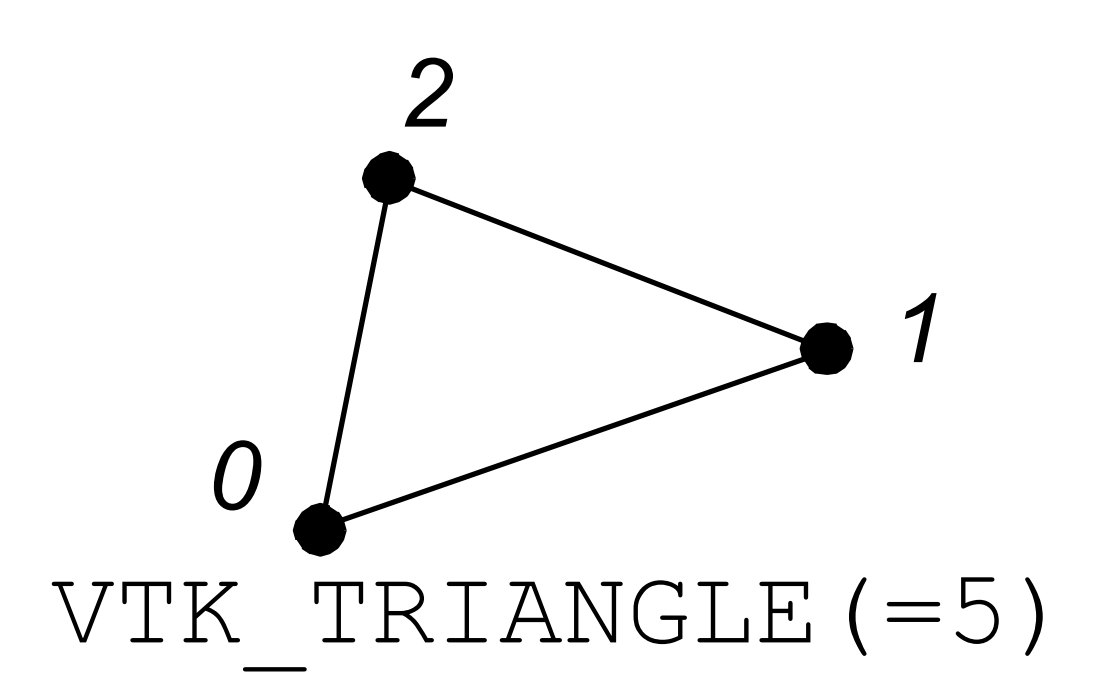
\includegraphics[width=0.3\textwidth]{vtk_triangle}
        \caption{VTK description of triangle element.}
        \label{fig:vtk_triangle}
      \end{figure}
      The reference triangle $T_{ref}$ is located in
      $\xi \in [0,1]$ and $\eta \in [0,1-\xi]$. The basis functions for the 
      reference linear triangle are provided.
      \begin{align}
        \basis_1(\xi,\eta) &= \xi \\
        \basis_2(\xi,\eta) &= \eta \\
        \basis_3(\xi,\eta) &= 1-\xi-\eta
      \end{align}
      
      Originally proposed in \cite{textbookwhite}, there are simple expressions
      for the quantities. The expression for the line integral is found in 
      \cite{computerLab}. For a triangle with corners $\{ x_i,y_i \}$.
      \begin{align}
        \int_{\Omega_e} \grad \basis_i(\vr) \cdot \grad \basis_j(\vr) 
          \;d\Omega_e &= \frac{1}{4 A_e}
          ((x_{i+1}-x_{i+2})(x_{j+1}-x_{j+2}) + 
          (y_{i+1}-y_{i+2})(y_{j+1}-y_{j+2})) \\
        \int_{\Omega_e} \basis_i(\vr) \basis_j(\vr) \;d\Omega_e &= 
          \frac{A_e}{12} (1+\delta_{ij}) \\
        \int_{\Omega_e} \basis_i(\vr) \;d\Omega_e &= \frac{A_e}{3} \\
        \int_{\partial \Omega_e} \basis_i(\vr) \basis_j(\vr) \;ds &=
          \frac{L_e}{6}(1+\delta_{ij}) 
      \end{align}
      Where $A_e$ is the area of the triangular element $L_e$ is the length of 
      the edge between node $i$ and node$j$, and $\delta_{ij}$ is the Kronecker
      delta such that
      \begin{equation} \label{eq:kroneker_delta}
        \delta_{ij} =
        \begin{cases}
          0 & \text{if } i \ne j \\
          1 & \text{if } i = j
        \end{cases}
      \end{equation}
      For higher order triangular elements, it will be necessary to employ a 
      quadrature.
    \subsubsection{Linear Wedges}
      Wedge elements have not reached the same commonality as triangular 
      elements but are extruded triangles. Geometrically, the shape is a 
      pentahedron or a triangular prism. However, their exact geometric
      relation is not fixed and the nodes are free to expand. These shapes 
      are unique because three of the faces are quadrilateral and two of
      the faces are triangular. The wedge from the VTK toolkit is described in
      \fref{fig:vtk_wedge} \cite{vtk}.
      \begin{figure}
        \centering
        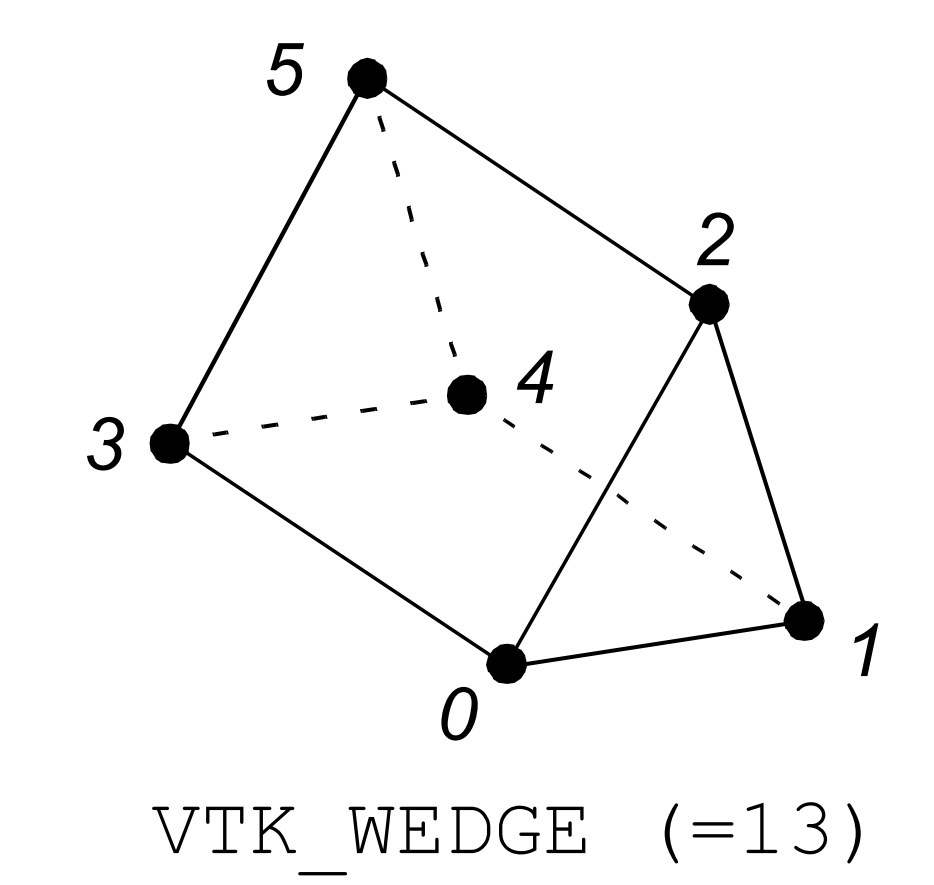
\includegraphics[width=0.3\textwidth]{vtk_wedge}
        \caption{VTK description of wedge element.}
        \label{fig:vtk_wedge}
      \end{figure}
      The reference wedge $W_{ref}$ is located in 
      $\xi \in [0,1]$, $\eta \in [0,1-\xi]$, and $\zeta \in [-1,1]$. The basis
      functions for the reference wedge are provided.
      \begin{align}
        \basis_1(\xi,\eta,\zeta) &= \half (1-\zeta)(1-\xi-\eta) \\
        \basis_2(\xi,\eta,\zeta) &= \half (1-\zeta)\xi \\
        \basis_3(\xi,\eta,\zeta) &= \half (1-\zeta)\eta \\
        \basis_4(\xi,\eta,\zeta) &= \half (1+\zeta)(1-\xi-\eta) \\
        \basis_5(\xi,\eta,\zeta) &= \half (1+\zeta)\xi \\
        \basis_6(\xi,\eta,\zeta) &= \half (1+\zeta)\eta 
      \end{align}
      The values presented herein are not yet found in literature and are 
      calculated by there author and published here for the first time.
      \begin{align}
        \int_{\Omega_e} \basis_i(\vr) \basis_j(\vr) \;d\Omega_e &= 
          \frac{V_e}{2}
          \begin{pmatrix}
            \frac{1}{18} & \frac{1}{36} & \frac{1}{36} & \frac{1}{36} & 
              \frac{1}{72} & \frac{1}{72} \\
            \frac{1}{36} & \frac{1}{18} & \frac{1}{36} & \frac{1}{72} & 
              \frac{1}{36} & \frac{1}{72} \\
            \frac{1}{36} & \frac{1}{36} & \frac{1}{18} & \frac{1}{72} & 
              \frac{1}{72} & \frac{1}{36} \\
            \frac{1}{36} & \frac{1}{72} & \frac{1}{72} & \frac{1}{18} & 
              \frac{1}{36} & \frac{1}{36} \\
            \frac{1}{72} & \frac{1}{36} & \frac{1}{72} & \frac{1}{36} & 
              \frac{1}{18} & \frac{1}{36} \\
            \frac{1}{72} & \frac{1}{72} & \frac{1}{36} & \frac{1}{36} & 
              \frac{1}{36} & \frac{1}{18} 
          \end{pmatrix} \\
        \int_{\Omega_e} \basis_i(\vr) \;d\Omega_e &= \frac{V_e}{12} \\
        \int_{\partial \Omega_e} \basis_i(\vr) 
          \basis_j(\vr) \;d\partial\Omega_e &= 
          \begin{cases}
            \frac{A_{\Delta}}{12}(1+\delta_{ij}) & \text{if triangle} \\
            \frac{A_{\Box}}{36}(1+\delta_{ij})(1-\half \delta_{i,(5-j)}) &
              \text{if quadrilateral}
          \end{cases}
      \end{align}
      Where $V_e$ is the volume of the element. This matrix is indexed $A_{ij}$
      and is presented as a matrix because of its irregular form. Notice the 
      integral containing the gradient operator has been omitted because if 
      it could be computed analytically, it would be less computationally 
      efficient than using a quadrature.
      
  \subsection{Quadratures}
    \label{sec:quadratures}
    Quadratures are sets of coordinates and weights which allow for the exact 
    integration of polynomials of given order. For a given set of weights 
    $\{w_i\}$ and a set of coordinates $\{\vx\}$, the quadrature can be 
    expressed as follows.
    \begin{equation}
      \int_{\Omega} f(\vx) \;d\Omega \approx \sum_{i=1}^{N} w_i f(\vx_i)
    \end{equation}
    where $\Omega$ is an arbitrary domain described by $\{\vx_i\}$. The above
    quadrature will exactly integrate a polynomial of the order of the 
    quadrature. It is not necessarily true that $N$ be the order of the 
    quadrature.
    
    For one dimensional integrals, the Gaussian quadrature is common and the 
    most compact quadrature. The Gaussian quadrature exactly integrates a 
    polynomial of order $n$ using exactly $n$ points. Weights and coordinates
    for this quadrature set are presented in \cite{gaussianQuadrature}. For this
    quadrature, $n=N$.
    
    Two dimensional and three dimensional quadratures are necessary for the 
    solution of this problem. Triangular quadratures are not as simply derived 
    as line quadratures and the number of points need not equal the order of the
    polynomial integrated. The triangular quadrature as implemented here is 
    symmetric and open. That is, there are no points on the boundary of the 
    triangle. The structure for this triangular quadrature is found in 
    \cite{triangleQuadrature}.
    
    Quadrilateral quadrature sets are simply tensor products of two line 
    Gaussian quadratures. For an order $N$ polynomial, now $n^2$ points are 
    required. 
    
    Wedge quadrature sets are simply tensor products of a line Gaussian 
    quadrature and a triangular quadrature. 
    
    Basis functions are polynomials of first, second, or third order. These 
    quadratures are capable of exactly integrating functions of given order so 
    there is a quadrature order that will exactly integrate the Finite Element 
    quantities to the precision of the quadrature and the numeric precision. The
    table of the order required for exact integration are provided in 
    \tref{tab:quadrature_orders}.
    \begin{table}
      \caption{Quadrature orders for FEM quantities.}
      \label{tab:quadrature_orders}
      \begin{center}
        \begin{tabular}{lccc}
          \toprule
          Quantity & Linear & Quadratic & Cubic \\
          \midrule
          $\int_{\Omega} \basis_i(\vr) \;d\Omega$ & 1 & 2 & 4\footnotemark \\
          $\int_{\Omega} \basis_i(\vr) \basis_j(\vr) \;d\Omega$ &
            2 & 4 & 6 \\
          $\int_{\Omega} \grad \basis_i(\vr) \cdot \grad \basis_j(\vr) 
            \;d\Omega$ & 2 & 3 & 5 \\
          \bottomrule
        \end{tabular}
      \end{center}
    \end{table}
    \footnotetext{A third order quadrature would be exact but the quadrature
    would have negative weights so a fourth order quadrature is 
    selected.}
    
    All of the quadratures described here are tabulated for a reference element
    be it a line, a triangle, a quadrilateral, or a wedge. Integration in the 
    FEM is performed on an arbitrary element in space. Therefore, it is 
    necessary to perform a coordinate transform when using a quadrature set.
    \begin{equation}
      \int_{\Omega} f(\vx) \;d\Omega = 
        \int_{\Omega_{ref}} f(\vx) \lvert \mj \rvert \;d\Omega \approx
        \sum_{i=1}^{N} w_i f(\vx_i) \lvert \mj_i \rvert
    \end{equation}
    where $\mj$ is the Jacobian matrix, $\mj_i$ is the Jacobian matrix at 
    quadrature coordinate $\vx_i$, and $\lvert \cdot \rvert$ represents
    the matrix determinant. Notationally, $J=\lvert \mj \rvert$ and is termed
    the Jacobi.
    
    For simple elements, the Jacobi is constant over the element and can be
    precalculated to save from allocating, populating, and taking the 
    determinant of a matrix for each integration point. For the elements of 
    concern, these values are presented in \tref{tab:jacobi} as found in 
    \cite{textbookcolorado}.
    \begin{table}
      \caption{Jacobi for selected elements}
      \label{tab:jacobi}
      \begin{center}
        \begin{tabular}{ll}
          \toprule
          Element & $J$ \\
          \midrule
          Triangle      & $A_e$ \\
          Quadrilateral & $\frac{1}{4} A_e$ \\
          Wedge         & $\half V_e$ \\
          \bottomrule
        \end{tabular}
      \end{center}
    \end{table}

\section{Implementation}
  A Finite Element neutron diffusion solution method has been developed using 
  the above formulae. The program begins with a geometry description specified
  in a plaintext VTK file. Cross sections are specified in either a plaintext
  user format or the ISOTXS format as common to fast reactor applications 
  and the multigroup cross section generator \mcc. The multigroup neutron 
  diffusion equation is then solved according to \eref{eq:multigroup_source}.
  The resulting effective neutron multiplication factor, $\keff$, is written to
  an output file. The multigroup neutron flux is written to a different results
  VTK file for easy visualization.
  \subsection{Algorithm}
    The algorithm for this solution to the diffusion equation is similar to most
    implementations of the multigroup method. The algorithm itself is presented 
    in Algorithm \ref{algorithm:general}. The steps unique to the Finite Element
    method are steps \ref{state:fem_matrix} and \ref{state:fem_vector}. These
    require the quantities previously derived and form the linear system 
    described by the FEM. 
    
    In step \ref{state:rcm} the matrix is reordered. Mathematically this has no
    effect on the result as the linear system represented is equivalent. This 
    choice to reorder the system is made to improve computational efficiency. 
    Indexing nodes that are physically proximate with proximate indices causes 
    rows in the Finite Element Matrix $\ma$ to be closely coupled to nearby
    rows. In a general unstructured and unordered mesh rows may be coupled to 
    other random rows in the matrix. This step of reordering the matrix $\ma$ 
    seeks to decrease the bandwidth of the matrix and encourage cache hits when
    accessing coupled values in the linear system. The ordering chosen is the
    Reverse Cuthill-McKee (RCM) method and common to sparse linear systems and 
    described in \cite{rcm}.
    
    \begin{algorithm}
      \caption{General Iteration Scheme}
      \label{algorithm:general}
      \begin{algorithmic}[1]
      \State Initialize $\phiavg^{(0)}$.
      \State Order the nodes of the mesh into RCM order \cite{rcm}. 
        \label{state:rcm}
      \State Calculate $\Sigma_s$, $\Sigma_t$, and $\nu \Sigma_f$ for each 
        element.
      \State Calculate Finite Element Matrix $\ma_g$ for each group. Store this. 
        \label{state:fem_matrix}
      \While{Power Iteration}
      	\State Update the iteration counter. $s=s+1$
      	\State Update $q_{fiss}$ and $q_{up}$ from previous data
          $\phiavg^{(s-1)}$.
        \State Update $\chi$ in each element using previous data
        \For{$g=1,G$}
          \State Update $q_{down}$ from current data $\phiavg^{(s)}$
          \State Calculate total effective source in each element.
          \State Update Finite Element Vector $\vf_g$ with new source.
            \label{state:fem_vector}
          \State Solve $\ma \vu = \vf$ using an iterative technique.
          \State Parse $\vu$ for $\phi$ nodal solution.
          \State Calculate element-average $\phiavg$.
        \EndFor
        \State Update $k_{eff}$.
        \State Check convergence.
      \EndWhile
      \end{algorithmic}
    \end{algorithm}
    
    Note that the Finite Element vector $\vf$ must be updated on each iteration
    of the solution whereas the matrix $\ma$ is described entirely by geometry 
    and the material cross sections. For this reason, $\ma$ can be generated 
    once at the beginning of the problem and stored for the duration of the 
    calculation.
    \FloatBarrier % make sure the algorithm is in the correct section
  \subsection{Memory and Storage}
    The Finite Element matrix $\ma$ is large and sparse so a sparse storage and
    sparse solution to the linear system are required. Many sparse matrix 
    implementations have been described and implemented in the past including
    triplet storage, reduced column, and reduced row storage \cite{sparseBLAS}.
    For this application a \twotable method is chosen which was uniquely 
    developed. \twotable storage is not designed to be the most efficient 
    storage method but is chosen for its simplicity and conforming with the 
    FEM. Future work may include a reduced row implementation but there will be
    a tradeoff between memory minimization and computational efficiency.
    
    The \twotable method is composed of two separate matrices in memory. An 
    integer index table, \texttt{IDX}, and a double precision value table
    \texttt{VAL}. Each table is dimension $DOF \times D$ where $DOF$ is the
    number of degrees of freedom of the linear system and $D$ is the maximum
    number of nodes that a node shares including itself. This must be determined
    a priori. 
    
    \texttt{IDX} is initialized to -1 and \texttt{VAL} is initialized 
    to 0.0 such that an index of -1 corresponds to a zero entry in the 
    matrix. \texttt{IDX} is then populated with a modified adjacency graph. 
    Values in \texttt{IDX} indicate the column in which the \texttt{VAL} entry
    occurs. For example, the following descriptions are equivalent.
    \begin{align}
      \texttt{IDX}(7,3) &= 8 \\
      \texttt{VAL}(7,3) &= 12.0 \\
      A_{7,8} &= 12.0
    \end{align}
    All of these representations indicate that the value of matrix $\ma$ in the
    seventh row in the eighth column is 12.0. This will allow for simple row 
    operations and matrix vector multiplication which will be necessary in the 
    solution of the system.
    
  \subsection{Boundary Conditions}
    Boundary conditions deserve brief consideration. There are many way to treat 
    sets of boundary conditions and all result in mathematically the same 
    answer. The choices made for this application are presented below. Mirror 
    boundary conditions require $\grad \phi_g(\vr) = 0$ for 
    $\vr \in \partial \Omega$. These are also known as ``natural'' boundary
    conditions because the Finite Element Matrix $\ma$ requires no additional 
    treatment and this condition is natural.
    
    Albedo boundary conditions are treated with an additional contribution to 
    the Finite Element Matrix $\ma$. These contributions represent a line 
    integral in two dimensions and a surface integral in three dimensions. These
    values are found in \eref{eq:matrix_population} and the quantities are 
    expressed in \sref{sec:matrix_quantities} or by quadratures 
    \sref{sec:quadratures}.
    
    Zero Flux boundary conditions require $\phi(\vr) = 0$ for 
    $\vr \in \partial \Omega$. These are treated by removing these entries from
    the Finite Element Matrix $\ma$. Entries are removed by using an index 
    vector. In a natural system (see Mirror boundary conditions above) each node
    corresponds to a row/column of the matrix. With entries removed, node number
    and index number may not exactly agree. A vector \texttt{ID} is introduced
    \cite{textbookjohnson}. Nodes with non-zero flux boundary conditions are set
    to a sequential positive integer. Nodes with zero flux boundary conditions 
    are set to a negative integer (-1) and are omitted in the actual solution of 
    the system. Other strategies have been proposed such as the penalty approach 
    \cite{textbookhughes} and manually forcing the solution of the linear system 
    \cite{textbookli}. This method is chosen because it decreases the degree of 
    freedom of the linear system while encouraging a well conditioned matrix. 
    Now, the degree of freedom of the matrix is equal to the number of nodes 
    with non-zero flux boundary conditions.
    
  \subsection{Linear System Solution}
    For a nonsingular linear system $\ma \vu = \vf$, where $\ma$ is a square 
    matrix, there exists a unique solution. Many strategies have been proposed 
    to solve this system in an efficient manner. Options are restricted in this
    application because the solution must operate with a sparsely stored linear 
    system and result in no fill-in. This immediately demands an iterative 
    method. The linear system described by the FEM can then be exploited for its 
    unique properties to select a favorable solution method.
    
    The Finite Element Matrix $\ma$ for the problem described in 
    \eref{eq:multigroup_source} is Symmetric Positive Definite (SPD). Symmetry
    condition is straight-forward and is observed in the elemental matrix 
    description \eref{eq:matrix_population}. Briefly, $A_{i,j,g,e}=A_{j,i,g,e}$.
    Positive definiteness is a particularly useful condition but is often 
    difficult to prove. $\ma$ is sometimes diagonally dominant for conveniently
    ordered meshes and certain elements but generally the matrix is not 
    diagonally dominant. 
    
    A matrix $\ma \in \realnn$ is positive definite if
    \begin{equation} \label{eq:positive_definite}
      \vx^{T} \ma \vx > 0 \qquad \forall \vx \in \realn, \; \vx \ne 0
    \end{equation}
    Following the proof of Theorem 1.9 in \cite{textbookhughes}. Let 
    $\vx = \{x_i\}$ for $i = 1,2,\ldots,N$. Then the vector-matrix and 
    matrix-vector products can be rewritten as summations.
    \begin{equation}
      \vx^{T} \ma \vx = \sum_{i=1}^{N} \sum_{j=1}^{N} x_i A_{ij} x_j
    \end{equation}
    By the definition of $A_{ij}$ in \eref{eq:matrix_population} and 
    \eref{eq:fem_notation}.
    \begin{equation}
      \vx^{T} \ma \vx = 
        \sum_{i=1}^{N} \sum_{j=1}^{N} x_i a(\basis_i,\basis_j) x_j
    \end{equation}
    Noting the property that $a(\cdot,\cdot)$ is a bilinear operator (i.e.
    linear in both arguments) \cite{textbookli}.
    \begin{equation}
      \vx^{T} \ma \vx =
        a \left( \sum_{i=1}^{N} x_i \basis_i, \sum_{j=1}^{N} x_j \basis_j 
        \right)
    \end{equation}
    By construction of the FEM, $w(\vr) \sum_{i=1}^{N} x_i \basis_i$ where 
    $w(\vr)$ is a piecewise continuous polynomial of arbitrary order.
    \begin{equation}
      \vx^{T} \ma \vx = a \left(w(\vr),w(\vr)\right)
    \end{equation}
    $a(\cdot,\cdot)$ can be shown to form a norm $\|\cdot \|_a$ requiring the 
    positive definite condition \cite{textbookli}.
    \begin{equation}
      \vx^{T} \ma \vx > 0 \qquad \forall \vx \in \realn, \; \vx \ne 0
    \end{equation}
    This satisfies the positive definite condition from 
    \eref{eq:positive_definite}.
    
    A given matrix can be verified as positive definite by one of two methods.
    First, all eigenvalues of the matrix have positive real components. Second, 
    the matrix has a Cholesky decomposition such that $\ma = \ml \ml^*$ where 
    $\ml$ is a lower triangular matrix with positive diagonal entries and 
    $\ml^*$ is the conjugate transpose of the matrix \cite{textbookipsen}. For 
    real valued matrices, the conjugate transpose is equivalent to the 
    conventional transpose.
    
    Symmetric Positive Definite matrices also posses a unique inverse. 
    Conventional methods to solve a linear system described by an SPD matrix 
    include Gauss-Seidel iteration with Successive Over-Relaxation (SOR) and
    the Conjugate Gradient (CG) Krylov subspace method. SOR requires a priori 
    knowledge of the optimized  over-relaxation factor $\omega_{opt}$. In 
    practice, this is performed analytically with arbitrary and contrived 
    solutions or in a modified guess-and-check method. For this application, the
    CG method is chosen because it requires no a priori knowledge and produced
    a solution to the same tolerance in a comparable time without the need for 
    guess-and-check iterations.
    
    A simple recipe for the CG method is presented in Algorithm 2.4.1
    \cite{Kelley1995IterativeEquations} and its implementation in this 
    application is replicated in Algorithm \ref{algorithm:CG}.
    
    \begin{algorithm}
      \caption{Conjugate Gradient Method}
      \label{algorithm:CG}
      \begin{algorithmic}[1]
        \State $k = 0$
        \State $\vr = \vb - \ma \vx$
        \State $\rho_k = \|\vr\|_2^2$
        \State $k = k + 1$
        \While{$\sqrt{\rho_{k-1}} > \epsilon \|\vb\|_2$}
          \If{$k=1$}
            \State $\vp = \vr$
          \Else
            \State $\beta = \rho_{k-1} / \rho{k-2}$
            \State $\vp = \vr + \beta \vp$
          \EndIf
          \State $\vw = \ma \vp$
          \State $\alpha = \rho_{k-1} / \vp^{T} \vw$
          \State $\vx = \vx + \alpha \vp$
          \State $\vr = \vr - \alpha \vw$
          \State $\rho_k = \| \vr \|_2^2$
          \State $k=k+1$
        \EndWhile
      \end{algorithmic}
    \end{algorithm}
    
    Where $\epsilon$ is a tolerance set by the user and the square of the 
    two-norm is most efficiently replaced by the inner-product. It is noted 
    that this method requires minimal storage with only four vectors 
    required ($\vx, \vw, \vp,$ and $\vr$). Additionally, two scalar products 
    are required and a matrix-vector product which proves to be the most 
    computationally expensive \cite{Kelley1995IterativeEquations}. As most of 
    the computational time of the diffusion solutions is spent in the linear 
    system solution, is is crucial that this process be efficient.

\section{Reference Results}
  This application of the FEM has been benchmarked against reference 
  reactor-type problems as well as contrived manufactured solutions. Comparison
  against reactor-type problems demonstrates an ability to solve problems for
  which this method was derived. Comparison against manufactured solutions 
  allows for more detailed error and convergence analysis as not only the system
  $\keff$ but also the exact flux solution is known.
  
  For all reference problems presented, a convergence study is presented. It has 
  been shown that for a bounded second spatial derivative within the problem 
  domain, the FEM derived above is second order convergent \cite{textbookli} 
  (Remark 7.13).
  \begin{equation} \label{eq:error_bound}
    \|\ve\|_{\infty} \le c h^2 \| \grad^2 \phi(\vr) \|_{\infty}
  \end{equation}
  Where $\ve$ is the error vector such that $\ve = \phi(\vr) - \phi_{FEM}$ and
  $\phi_{FEM}$ is solution to the finite element system of equations. Then,
  $h$ is the characteristic mesh size, and $c$ is a constant. 
  \eref{eq:error_bound} implies that if a characteristic mesh size is halved, 
  the error is quartered. This relationship is useful as a proper implementation 
  of the FEM will converge to the correct answer and do so at the correct rate.
  
  Mesh refinement studies are presented herein. For each refinement, $h$ is 
  halved by introducing new elements and placing new nodes at the midway point
  between existing nodes. Then, let $r$ be the refinement index.
  \begin{equation}
    x = 4 = \frac{x^{(r-1)}}{x^{(r)}}
  \end{equation}
  Such that for some quantity $x$, the error decreases by a factor of four for 
  each refinement. As these are numerical solutions, the ratio rarely equals 
  exactly four. It is observed that a few refinements are often necessary 
  before the ratio approaches the expected value. This is especially the case
  when the second derivative is not bounded in problems with heterogeneous 
  materials.
  
  For reactor-type problems, only $\keff$ is analyzed and expected to converge
  at the appropriate rate. When assembly powers were available, these are also
  presented graphically. In the graphical power representation, the key is 
  presented in \fref{fig:hex_description}.
  \begin{figure}
    \centering
    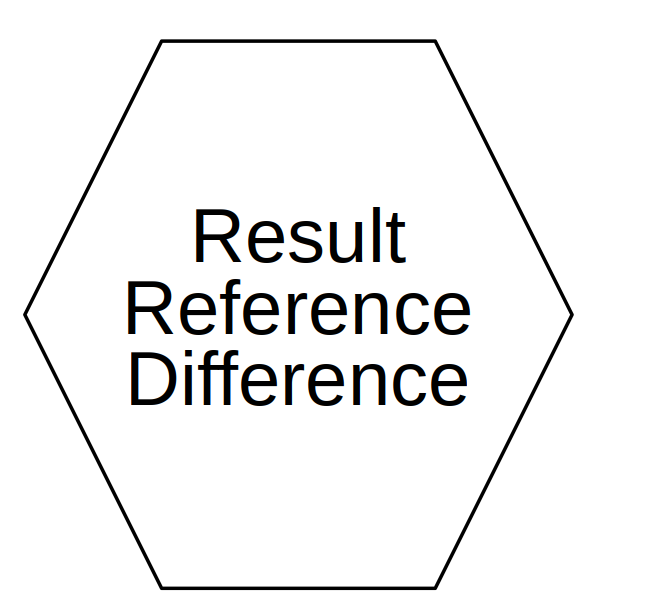
\includegraphics[width=0.25\textwidth]{hex_description}
    \caption{Key for hexagonal power plots.}
    \label{fig:hex_description}
  \end{figure}
  
  For manufactured solutions, the error of the function $\phi$ itself can be 
  analyzed because the function is known exactly. The derivations of the exact 
  functions are presented in \apref{ap:analyticSolutions}. Equations are 
  presented here but their derivations are in the appendix. For all manufactured 
  problems, the Root Mean Squared (RMS) error as in \eref{eq:rms} is calculated
  for the error vector $\ve$ and is presented. The ratio between refinements 
  should assume the expected rate.
  \begin{equation} \label{eq:rms}
    \text{RMS}(\ve) = \sqrt{\frac{1}{N} \sum_{i=1}^{N} e_i}
  \end{equation}
  The maximal norm $\| \cdot \|_{\infty}$ is also presented and the ratio 
  between refinements should assume the expected value.
  \begin{equation} \label{eq:infnorm}
    \|\ve\|_{\infty} = \max_{i=1,2,\ldots,N} \lvert e_i \rvert
  \end{equation}
  For criticality  problems, $\keff$ is also presented.
  
  \subsection{Triangular Element Manufactured Solutions}
    As a demonstration of the proper implementation of and solution to the 
    diffusion equation for triangular elements, manufactured solutions are 
    derived and then numerically computed. These are One and Two Dimension 
    problems. All of these are on a rectangular domain $[0,L_x] \times [0,L_y]$.
    For One Dimension problems, the edges $y=0$ and $y=L_x$ are mirror boundary 
    conditions to reduce the dimension of the problem.
    \subsubsection{One Dimension, One Group, Fixed Source}
      \label{sec:1dfixedsrc}
      Arguably the simplest solutin to the neutron diffusion equation, this 
      problem  solves a domain $x \in [0,1]$ for a fixed unit source throughout
      the  problem. The exact solution is derived in \sref{sec:deriv_1dfixedsrc}
      and the solution is presented in \eref{eq:analytic_1dfixedsrc}. Results 
      from the convergence study are presented in \tref{tab:1dfixedsrc}.
      \begin{table}
        \caption{One Dimension, One Group, Fixed Source Convergence Study 
          Results.}
        \label{tab:1dfixedsrc}
        \begin{center}
          \begin{tabular}{ccccc}
            \toprule
            Refine & RMS & RMS ratio & $\|e\|_{\infty}$ & 
              $\|e\|_{\infty}$ ratio \\
            \midrule
            \csvreader[
              late after line=\\,
              late after last line=\\\bottomrule,]
              {ch02_neutronDiffusion/data/1dfixedsrc.csv}{}
              {\csvcoli & \csvcolii & \csvcoliii & \csvcolviii & \csvcolix}
          \end{tabular}
        \end{center}
      \end{table}
    \subsubsection{One Dimension, One Group, Criticality}
      \label{sec:1d1g}
      In addition to the fixed source problem in \sref{sec:1dfixedsrc}, this 
      problem tests the calculation of the source term and the general iteration
      implementation in the solution method. This problem solves a fissile 
      material in the domain $x \in [0,100]$.
      The exact solution is derived in \sref{sec:deriv_1d1g} and
      the solution is presented in \eref{eq:analytic_1d1g}. Results from
      the convergence study are presented in \tref{tab:1d1g}. The exact value 
      for the effective multiplication factor is $k_{ref} = 1.9980280254$.
      \begin{table}
        \caption{One Dimension, One Group, Criticality Convergence Study
          Results. $k_{ref} = 1.9980280254$}
        \label{tab:1d1g}
        \begin{center}
          \begin{tabular}{cccccccccc}
            \toprule
            Refine & $\keff$ & $\keff$ error \units{pcm} & $\keff$ ratio & RMS & 
              RMS ratio  & $\|e\|_{\infty}$ & $\|e\|_{\infty}$ ratio \\
            \midrule
            \csvreader[
              late after line=\\,
              late after last line=\\\bottomrule,]
              {ch02_neutronDiffusion/data/1d1g.csv}{}
              {\csvcoli & \csvcolii & \csvcoliii & \csvcoliv & \csvcolv & 
              \csvcolvi & \csvcolxi & \csvcolxii}
          \end{tabular}
        \end{center}
      \end{table}
    \subsubsection{Two Dimension, One Group, Criticality}
      In addition to the one dimension problem in \sref{sec:1d1g}, this problem
      tests the ability to solve truly two dimensional problems.
      The exact solution is derived in \sref{sec:deriv_2d1g} and
      the solution is presented in \eref{eq:analytic_2d1g}. Results from
      the convergence study are presented in \tref{tab:2d1g}. The exact value 
      for the effective multiplication factor is $k_{ref} = 1.9960599356$.
      \begin{table}
        \caption{Two Dimension, One Group, Criticality Convergence Study
          Results. $k_{ref} = 1.9960599356$}
        \label{tab:2d1g}
        \begin{center}
          \begin{tabular}{cccccccccc}
            \toprule
            Refine & $\keff$ & $\keff$ error \units{pcm} & $\keff$ ratio & RMS & 
              RMS ratio  & $\|e\|_{\infty}$ & $\|e\|_{\infty}$ ratio \\
            \midrule
            \csvreader[
              late after line=\\,
              late after last line=\\\bottomrule,]
              {ch02_neutronDiffusion/data/2d1g.csv}{}
              {\csvcoli & \csvcolii & \csvcoliii & \csvcoliv & \csvcolv & 
              \csvcolvi & \csvcolxi & \csvcolxii}
          \end{tabular}
        \end{center}
      \end{table}
    \subsubsection{One Dimension, Two Group, Criticality }
      In addition to the one group problem in \sref{sec:1d1g}, this problem
      tests the solution of mulitgroup problems. The results presented are the 
      convergece of $\keff$ and the ratio of relative magnitude of thermal to 
      fast flux $\phi_2/\phi_1$.
      The exact solution is derived in \sref{sec:deriv_1d2g} and
      the solutions are presented in \eref{eq:twogroupflux1} and
      \eref{eq:twogroupflux2}. Results from the convergence study are presented in 
      \tref{tab:1d2g}. The exact value for the effective multiplication factor 
      is $k_{ref} = 0.892349025$ and the exact value for the relative flux ratio
      is $(\phi_2/\phi_1)_{ref} = 0.26132419$.
      \begin{table}
        \caption{One Dimension, Two Group, Criticality Convergence Study
          Results. $k_{ref} = 0.892349025$ $(\phi_2/\phi_1)_{ref} = 0.26132419$}
        \label{tab:1d2g}
        \begin{center}
          \begin{tabular}{ccccccc}
            \toprule
            Refine & $\keff$ & $\keff$ error \units{pcm} & $\keff$ ratio & 
              $\phi_2/\phi_1$ & $\phi_2/\phi_1$ error & $\phi_2/\phi_1$ ratio \\
            \midrule
            \csvreader[
              late after line=\\,
              late after last line=\\\bottomrule,]
              {ch02_neutronDiffusion/data/1d2g.csv}{}
              {\csvcoli & \csvcolii & \csvcoliii & \csvcoliv & \csvcolv & 
              \csvcolvi & \csvcolvii}
          \end{tabular}
        \end{center}
      \end{table}
    \subsubsection{One Dimension, One Group, Two Region, Criticality}
      In addition to the homogenous problem in \sref{sec:1d1g}, this problem
      tests the mapping of materials to regions within the problem.
      The exact solution is derived in \sref{sec:deriv_2reg} and
      the solution is presented in \eref{eq:analytic_2reg}. Results from
      the convergence study are presented in \tref{tab:2reg}. The exact value 
      for the effective multiplication factor is $k_{ref} = 0.9621882561$.
      \begin{table}
        \caption{One Dimension, One Group, Two Region, Criticality Convergence
          Study Results. $k_{ref} = 0.9621882561$}
        \label{tab:2reg}
        \begin{center}
          \begin{tabular}{cccccccccc}
            \toprule
            Refine & $\keff$ & $\keff$ error \units{pcm} & $\keff$ ratio & RMS & 
              RMS ratio  & $\|e\|_{\infty}$ & $\|e\|_{\infty}$ ratio \\
            \midrule
            \csvreader[
              late after line=\\,
              late after last line=\\\bottomrule,]
              {ch02_neutronDiffusion/data/2reg.csv}{}
              {\csvcoli & \csvcolii & \csvcoliii & \csvcoliv & \csvcolv & 
              \csvcolvi & \csvcolxi & \csvcolxii}
          \end{tabular}
        \end{center}
      \end{table}
  \subsection{Two Dimension Reactors}
    \subsubsection{VVER440}
      Described by \cite{chao} this reactor-type two dimension problem is of
      VVER-440 type with 25 assemblies across the core diameter including an 
      outer reflector. The reactor has vacuum boundary conditions 
      ($\albedo = 0.5$). The core is simulated as a sixth-core problem with 
      mirror symmetry. Assembly pitch is $14.7 \units{cm}$. The VVER-440 is a 
      light-water moderated reactor and operates principally with thermal 
      neutrons. Cross sections are provided for a two-group energy structure.
      
      Power comparison between the most refined mesh and the reference solution 
      are presented graphically in \fref{fig:diffusion_vver440} according to the
      key in \fref{fig:hex_description}. Numerical mesh convergence study for 
      the quantity $\keff$ is presented in \tref{tab:vver440}.
      \begin{figure}
        \centering
        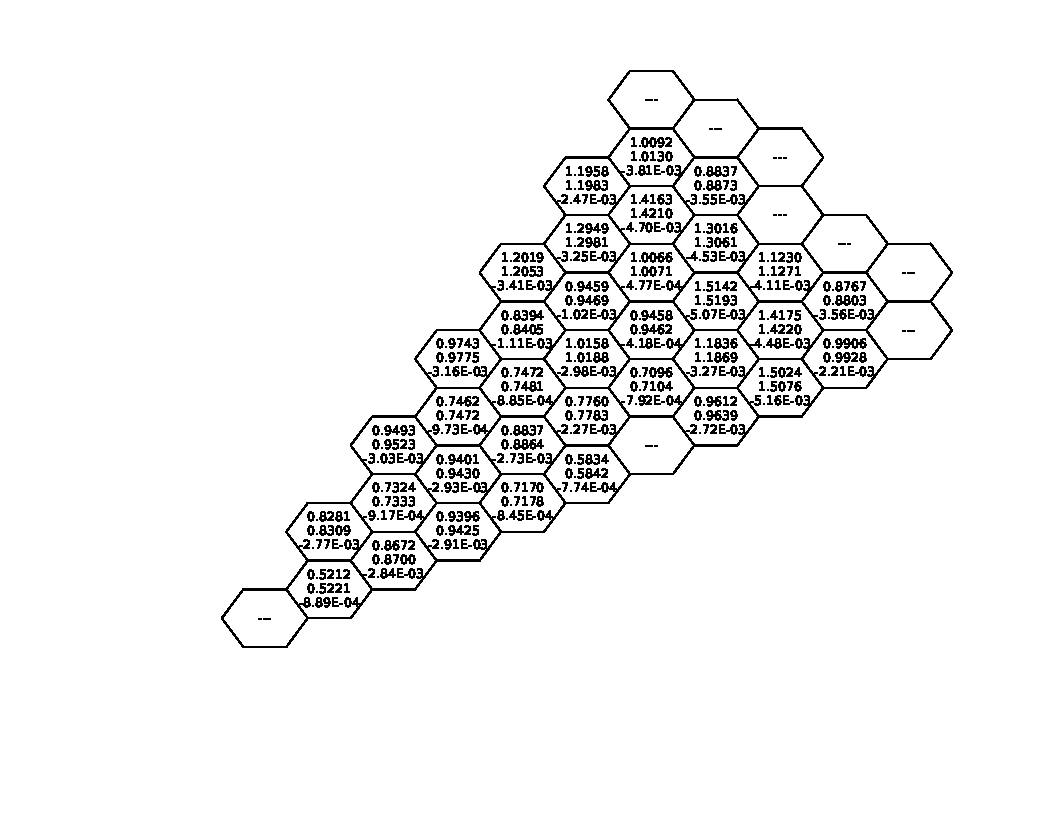
\includegraphics[width=\textwidth]{diffusion_vver440}
        \caption{VVER440 Benchmark Power Comparison for most refined mesh.}
        \label{fig:diffusion_vver440}
      \end{figure}
      \begin{table}
        \caption{VVER440 Benchmark Convergence Study. 
          $k_{ref} = 1.009700$ \cite{chao}}
        \label{tab:vver440}
        \begin{center}
          \begin{tabular}{cccc}
            \toprule
            Refine & $\keff$ & $\keff$ error \units{pcm} & $\keff$ ratio \\
            \midrule
            \csvreader[
              late after line=\\,
              late after last line=\\\bottomrule,]
              {ch02_neutronDiffusion/data/vver440.csv}{}
              {\csvcoli & \csvcolvi & \csvcolvii & \csvcolviii}
          \end{tabular}
        \end{center}
      \end{table}
    \subsubsection{SNR}
      \begin{figure}
        \centering
        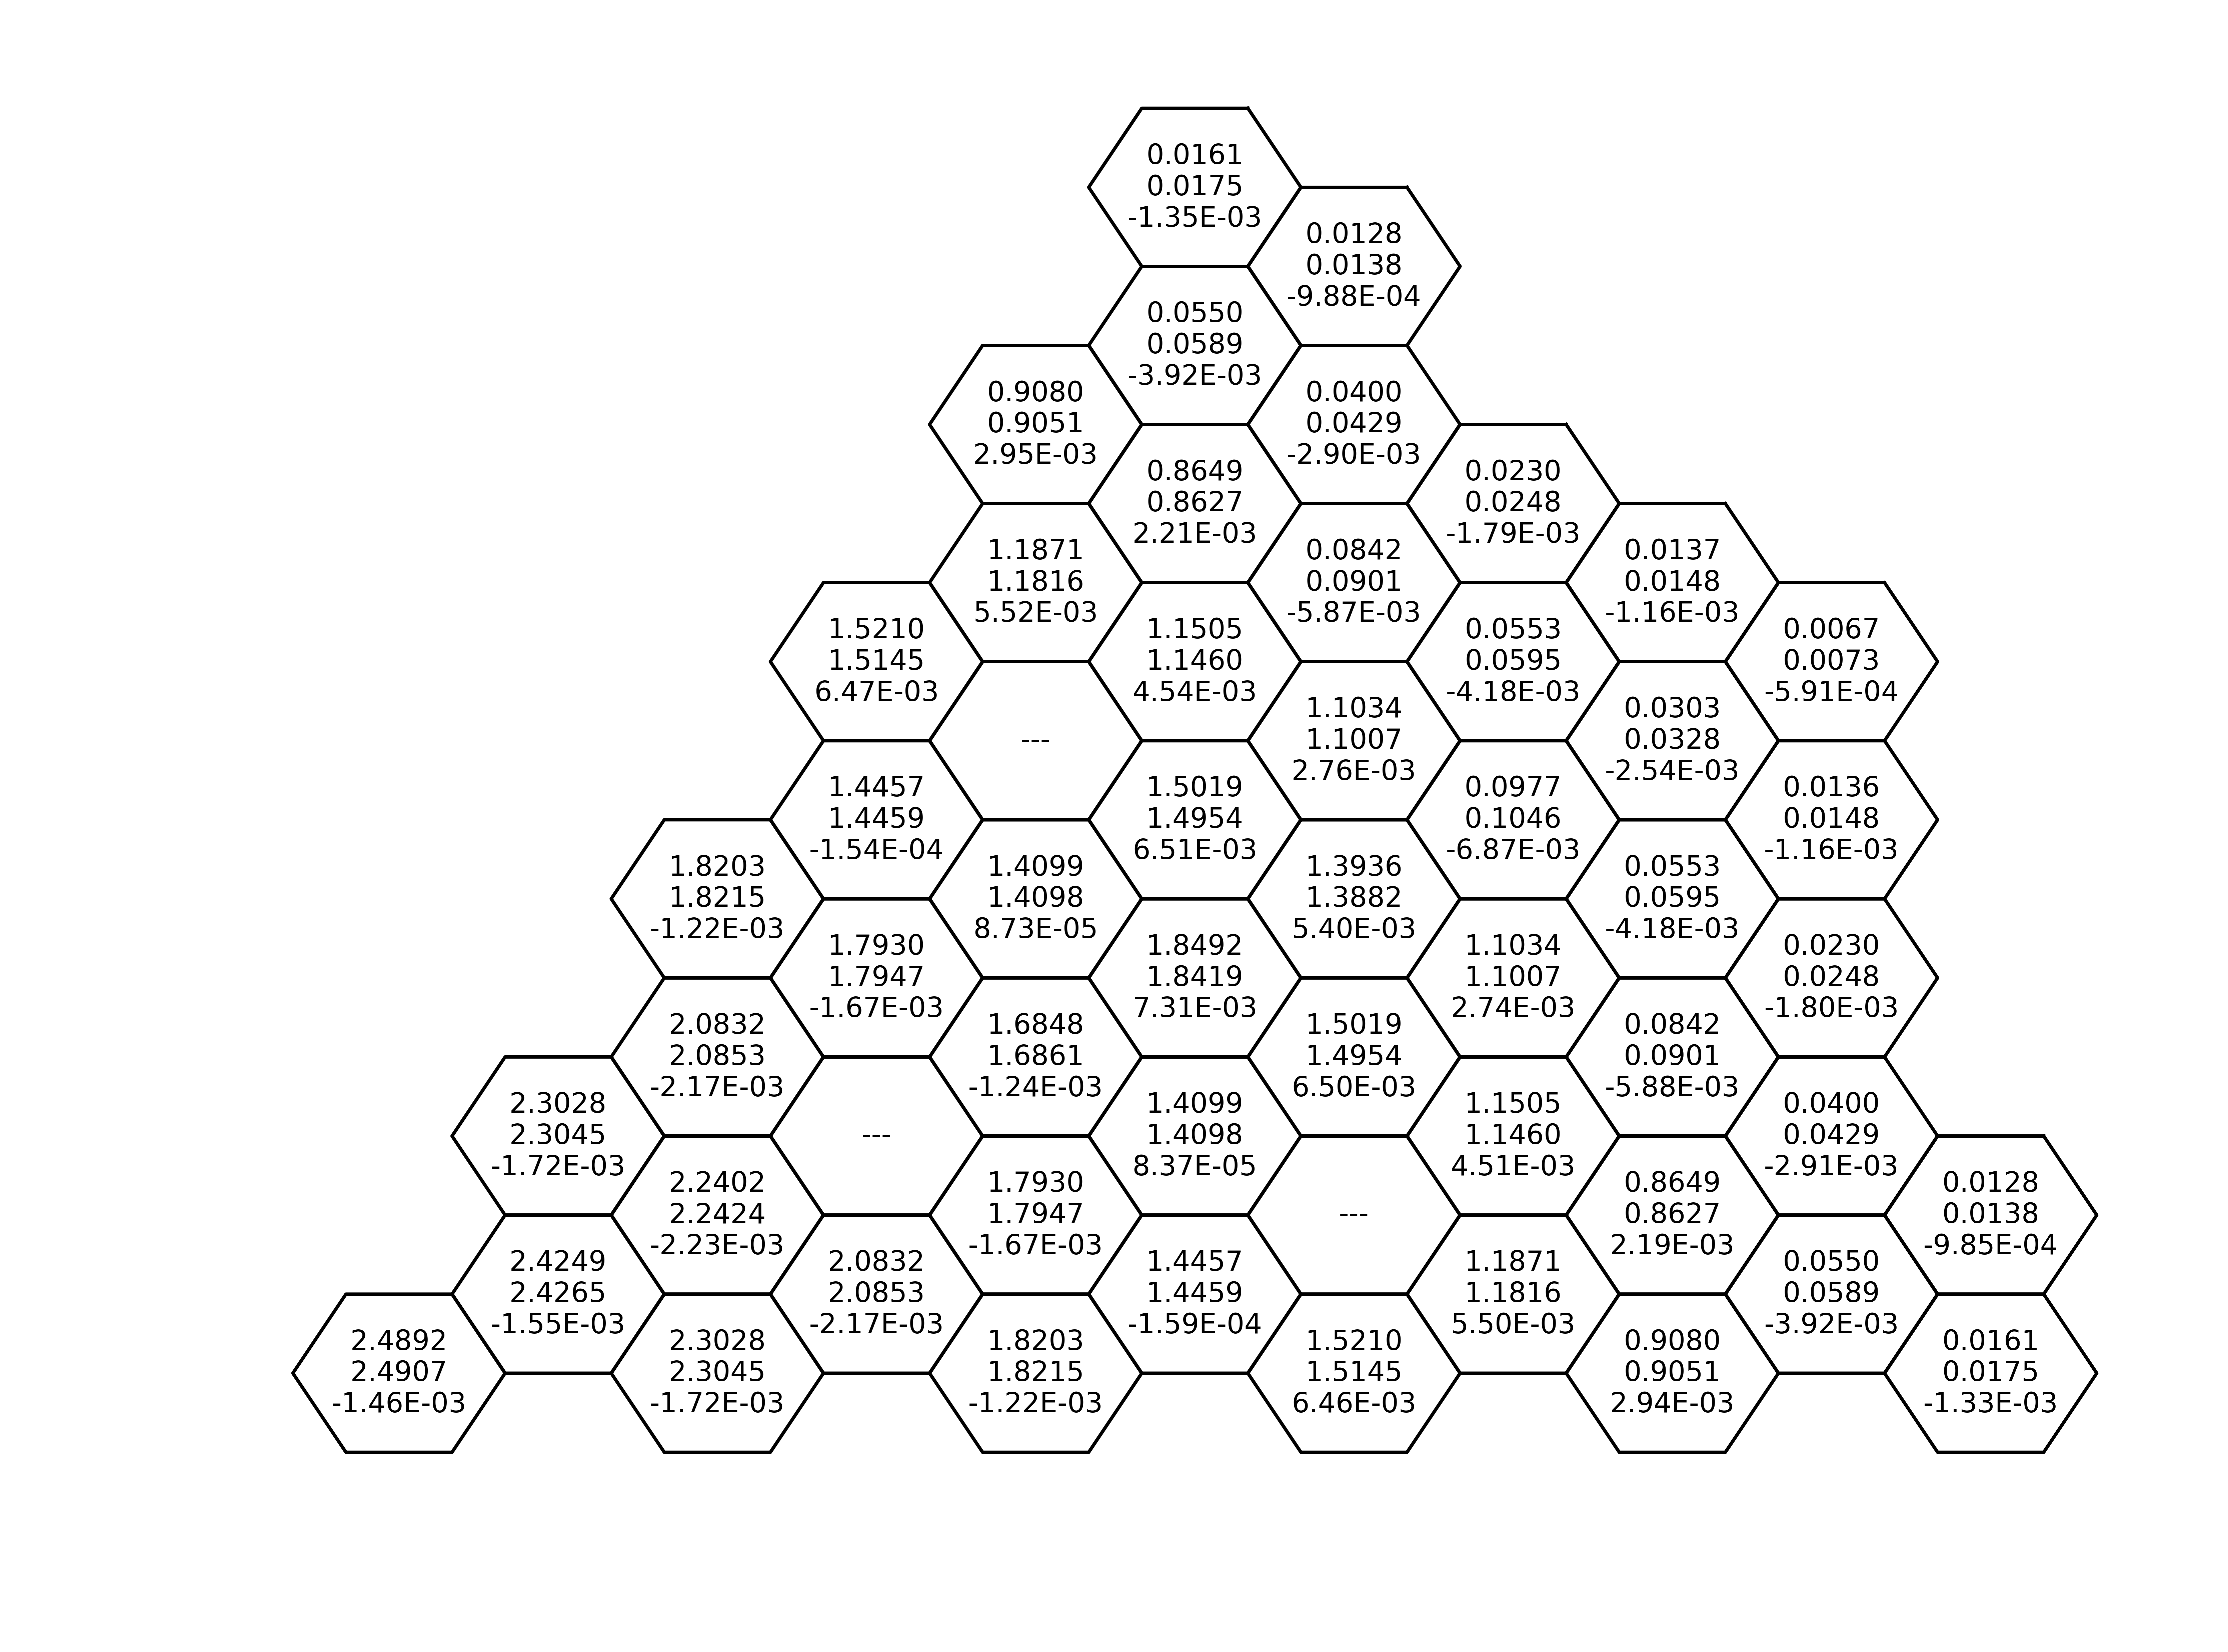
\includegraphics[width=\textwidth]{diffusion_snr}
        \caption{SNR Benchmark Power Comparison for most refined mesh.}
        \label{fig:diffusion_snr}
      \end{figure}
      \begin{table}
        \caption{SNR Benchmark Convergence Study. 
          $k_{ref} = 1.124000$ \cite{argonneBenchmark}}
        \label{tab:snr}
        \begin{center}
          \begin{tabular}{cccc}
            \toprule
            Refine & $\keff$ & $\keff$ error \units{pcm} & $\keff$ ratio \\
            \midrule
            \csvreader[
              late after line=\\,
              late after last line=\\\bottomrule,]
              {ch02_neutronDiffusion/data/snr.csv}{}
              {\csvcoli & \csvcolvi & \csvcolvii & \csvcolviii}
          \end{tabular}
        \end{center}
      \end{table}
    \subsubsection{HWR}
      \begin{figure}
        \centering
        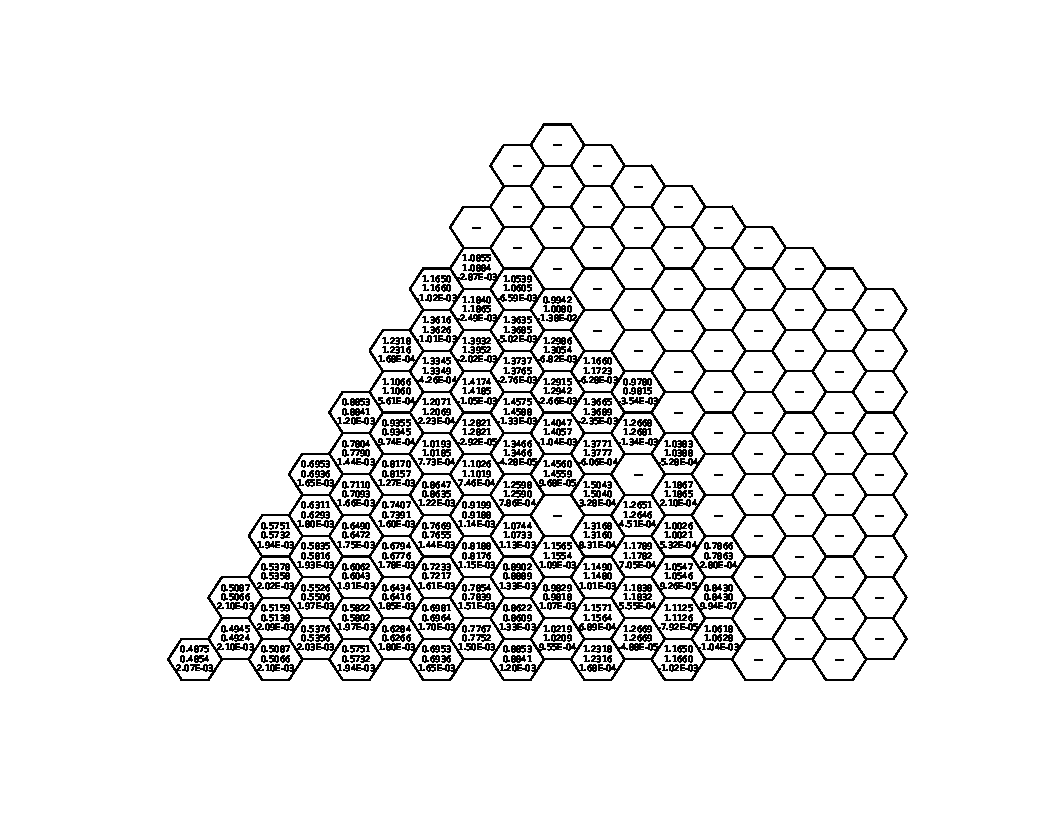
\includegraphics[width=\textwidth]{diffusion_hwr}
        \caption{HWR Benchmark Power Comparison for most refined mesh.}
        \label{fig:diffusion_hwr}
      \end{figure}
      \begin{table}
        \caption{HWR Benchmark Convergence Study. 
          $k_{ref} = 0.991965$ \cite{chao}}
        \label{tab:hwr}
        \begin{center}
          \begin{tabular}{cccc}
            \toprule
            Refine & $\keff$ & $\keff$ error \units{pcm} & $\keff$ ratio \\
            \midrule
            \csvreader[
              late after line=\\,
              late after last line=\\\bottomrule,]
              {ch02_neutronDiffusion/data/hwr.csv}{}
              {\csvcoli & \csvcolvi & \csvcolvii & \csvcolviii}
          \end{tabular}
        \end{center}
      \end{table}
    \subsubsection{IAEA}
      % nore0125
      \begin{table}
        \caption{IAEA Benchmark Convergence Study. No Reflector. $\albedo = 
          0.125$. $k_{ref} = 0.991378 $ \cite{chao}}
        \label{tab:iaea_nore0125}
        \begin{center}
          \begin{tabular}{cccc}
            \toprule
            Refine & $\keff$ & $\keff$ error \units{pcm} & $\keff$ ratio \\
            \midrule
            \csvreader[
              late after line=\\,
              late after last line=\\\bottomrule,]
              {ch02_neutronDiffusion/data/iaea_nore0125.csv}{}
              {\csvcoli & \csvcolvi & \csvcolvii & \csvcolviii}
          \end{tabular}
        \end{center}
      \end{table}
      % nore0500
      \begin{table}
        \caption{IAEA Benchmark Convergence Study. No Reflector. $\albedo = 
          0.500$. $k_{ref} = 0.978077$ \cite{chao}}
        \label{tab:iaea_nore0500}
        \begin{center}
          \begin{tabular}{cccc}
            \toprule
            Refine & $\keff$ & $\keff$ error \units{pcm} & $\keff$ ratio \\
            \midrule
            \csvreader[
              late after line=\\,
              late after last line=\\\bottomrule,]
              {ch02_neutronDiffusion/data/iaea_nore0500.csv}{}
              {\csvcoli & \csvcolvi & \csvcolvii & \csvcolviii}
          \end{tabular}
        \end{center}
      \end{table}
      % refl0125
      \begin{table}
        \caption{IAEA Benchmark Convergence Study. With Reflector. $\albedo = 
          0.125$. $k_{ref} = 1.006630 $ \cite{chao}}
        \label{tab:iaea_refl0125}
        \begin{center}
          \begin{tabular}{cccc}
            \toprule
            Refine & $\keff$ & $\keff$ error \units{pcm} & $\keff$ ratio \\
            \midrule
            \csvreader[
              late after line=\\,
              late after last line=\\\bottomrule,]
              {ch02_neutronDiffusion/data/iaea_refl0125.csv}{}
              {\csvcoli & \csvcolvi & \csvcolvii & \csvcolviii}
          \end{tabular}
        \end{center}
      \end{table}
      % refl0500
      \begin{table}
        \caption{IAEA Benchmark Convergence Study. With Reflector. $\albedo = 
          0.500$. $k_{ref} = 1.005507 $ \cite{chao}}
        \label{tab:iaea_refl0500}
        \begin{center}
          \begin{tabular}{cccc}
            \toprule
            Refine & $\keff$ & $\keff$ error \units{pcm} & $\keff$ ratio \\
            \midrule
            \csvreader[
              late after line=\\,
              late after last line=\\\bottomrule,]
              {ch02_neutronDiffusion/data/iaea_refl0500.csv}{}
              {\csvcoli & \csvcolvi & \csvcolvii & \csvcolviii}
          \end{tabular}
        \end{center}
      \end{table}
  \subsection{Wedge Element Manufactured Solution Finite Cylinder}
      A three dimension problem is presented that is contrived and has an 
      analytic solution. This problem is a finite cylinder with zero-flux
      boundary conditions. The cylinder is three dimensional but the solution
      can be reduced to two dimensions (radial and axial directions). 
      The exact solution is derived in \sref{sec:deriv_finite_cyl} and the
      solution is presented in \eref{eq:analytic_finite_cyl}. Results from the
      convergence study are presented in \tref{tab:finite_cyl}. The exact value
      for the effective multiplication factor is $k_{ref} = 0.996710620898177$.
      \begin{table}
        \caption{Finite Cylinder Convergence Study Results.
          $k_{ref} = 0.996710620898177$}
        \label{tab:finite_cyl}
        \begin{center}
          \begin{tabular}{cccccccccc}
            \toprule
            Refine & $\keff$ & $\keff$ error \units{pcm} & $\keff$ ratio & RMS & 
              RMS ratio  & $\|e\|_{\infty}$ & $\|e\|_{\infty}$ ratio \\
            \midrule
            \csvreader[
              late after line=\\,
              late after last line=\\\bottomrule,]
              {ch02_neutronDiffusion/data/finite_cyl.csv}{}
              {\csvcoli & \csvcolii & \csvcoliii & \csvcoliv & \csvcolv & 
              \csvcolvi & \csvcolxi & \csvcolxii}
          \end{tabular}
        \end{center}
      \end{table}
  \subsection{Three Dimension Reactors}
    \subsubsection{MONJU}
      \begin{table}
        \caption{MONJU Benchmark Rod Worth Results. \cite{monjuBenchmark}}
        \label{tab:monju}
        \begin{center}
          \begin{tabular}{ccll}
            \toprule
            Pattern & $\keff$ & Rod Worth \units{$\Delta k$} & 
              Rod Difference \units{\%$\Delta k$} \\
            \midrule
            \csvreader[
              late after line=\\,
              late after last line=\\\bottomrule,]
              {ch02_neutronDiffusion/data/monju.csv}{}
              {\csvcoli & \csvcolii & \csvcoliii \; \csvcolvi
              & \csvcoliv \; \csvcolvii}
          \end{tabular}
        \end{center}
      \end{table}
    \subsubsection{KNK}
      \begin{table}
        \caption{KNK Benchmark Rod Worth Results. \cite{takedaBenchmark}}
        \label{tab:knk}
        \begin{center}
          \begin{tabular}{ccll}
            \toprule
            Pattern & $\keff$ & Rod Worth \units{$\Delta k$} & 
              Rod Difference \units{\%$\Delta k$} \\
            \midrule
            \csvreader[
              late after line=\\,
              late after last line=\\\bottomrule,]
              {ch02_neutronDiffusion/data/knk.csv}{}
              {\csvcoli & \csvcolii & \csvcoliii \; \csvcolvi
              & \csvcoliv \; \csvcolvii}
          \end{tabular}
        \end{center}
      \end{table}
